% UQ Gemini theme
% See: https://github.com/alfurka/gemini-uq
% Forked from
% https://rev.cs.uchicago.edu/k4rtik/gemini-uccs
% which is forked from
% https://github.com/anishathalye/gemini


\documentclass[final]{beamer}

% ====================
% Packages
% ====================
\usepackage{lmodern}
\usepackage[size=a0]{beamerposter}
\usetheme{gemini}
\usecolortheme{uchicago}
\usepackage{graphicx}
\usepackage{booktabs}
\usepackage{tikz}
\usepackage{subcaption}
\usepackage{makecell}
\usepackage{caption}
\captionsetup[figure]{font=small,labelfont=small}
\captionsetup[table]{font=small,labelfont=small}
\usepackage{pgfplots}
\usetikzlibrary{shapes.geometric,shapes.multipart,arrows,positioning,calc,shapes.arrows,arrows.meta,pgfplots.statistics,backgrounds}
\pgfplotsset{compat=1.18}
\newcommand\smallimg{4cm}
\newcommand\smallerimg{3.5cm}
\newcommand{\tabfigure}[2]{\raisebox{-.5\height}{\includegraphics[#1]{#2}}}

\usepackage{array}
\newcolumntype{M}[1]{>{\centering\arraybackslash}m{#1}}

% ====================
% Lengths
% ====================

% If you have N columns, choose \sepwidth and \colwidth such that
% (N+1)*\sepwidth + N*\colwidth = \paperwidth
\newlength{\sepwidth}
\newlength{\colwidth}
\newlength{\twocolwid}
\setlength{\sepwidth}{0.024\paperwidth}
\setlength{\colwidth}{0.22\paperwidth}
\setlength{\twocolwid}{0.464\paperwidth} 

\newcommand{\separatorcolumn}{\begin{column}{\sepwidth}\end{column}}

% ====================
% Title
% ====================

\title{Active Visual Exploration Based on Attention-Map Entropy}

\author{Adam Pardyl \inst{1,2} \and
Grzegorz Rypeść \inst{1,3} \and
Grzegorz Kurzejamski \inst{1} \and
Bartosz Zieliński \inst{1,2,5} \and
Tomasz Trzciński \inst{1,2,3,4}}

\institute[shortinst]{
\inst{1} IDEAS NCBR \samelineand
\inst{2} Jagiellonian University \samelineand
\inst{3} Warsaw University of Technology \samelineand
\inst{4} Tooploox \samelineand
\inst{5} Ardigen
}

% ====================
% Footer (optional)
% ====================

\footercontent{
  \href{https://ideas-ncbr.pl/}{ideas-ncbr.pl} \hfill
  International Joint Conference on Artificial Intelligence (IJCAI) 2023, Macao, S.A.R. \hfill
  \href{mailto:adam.pardyl@ideas-ncbr.pl}{adam.pardyl@ideas-ncbr.pl}}
% (can be left out to remove footer)

% ====================
% Logo (optional)
% ====================

% use this to include logos on the left and/or right side of the header:
% \logoright{\includegraphics[height=7cm]{logo1.pdf}}
% \logoleft{\includegraphics[height=7cm]{logo2.pdf}}

% ====================
% Body
% ====================

\begin{document}
\addtobeamertemplate{headline}{}
{
    \begin{tikzpicture}[remember picture,overlay]
      \node [anchor=north west, inner sep=3cm] at ([xshift=0.0cm,yshift=0.5cm]current page.north west)
      {
\includegraphics[height=4.0cm]{fig/logos/ideas-logo.png}}; % also try shield-white.eps
      \node [anchor=north east, inner sep=3cm] at ([xshift=0.0cm,yshift=0.5cm]current page.north east)
      {\fontsize{140}{160}\selectfont\#2446};
    \end{tikzpicture}
}

\begin{frame}[t]
\begin{columns}[t]
\separatorcolumn

\begin{column}{\colwidth}

\begin{alertblock}{Abstract}

Active visual exploration addresses the issue of limited sensor capabilities in real-world scenarios, where successive observations are actively chosen based on the environment. To tackle this problem, we introduce a new technique called Attention-Map Entropy (AME). It leverages the internal uncertainty of the transformer-based model to determine the most informative observations. In contrast to existing solutions, it does not require additional loss components, which simplifies the training. Through experiments, which also mimic retina-like sensors, we show that such simplified training significantly improves the performance of reconstruction, segmentation and classification on publicly available datasets.

\end{alertblock}

\begin{block}{Active visual exploration}

\begin{figure}[th]
\begin{center}
\begin{scriptsize}
\begin{sc}
\begin{tikzpicture}[node distance=2ex, auto]
\tikzstyle{every node}=[font=\footnotesize]

\newlength{\stepimage}
\setlength{\stepimage}{6em}

\tikzstyle{module} = [rectangle, rounded corners, minimum width=2.5cm, minimum height=0.5cm,text centered, draw=black, fill=blue!20]
\tikzstyle{largemodule} = [rectangle, rounded corners, minimum width=3.5cm, minimum height=1cm,text centered, draw=black, fill=blue!20]
\tikzstyle{inputoutput} = [rectangle, rounded corners,text centered, draw=black,inner sep=5px]
\tikzstyle{arrow} = [ultra thick,->,>=stealth]
\tikzstyle{pict} = [inner sep=0px]

\node [module] (task) {\makecell[c]{Task:\\locate a predator}};

\node [inputoutput, left=of task] (human)  {
\includegraphics[height=3em]{fig_poster/overview/images/human.png}};
\node [inputoutput, right=of task] (robot)  {
\includegraphics[height=3em]{fig_poster/overview/images/robot.png}};

\node [pict, below=of human, label={[align=right]left:An animal\\on the left}] (h1)  {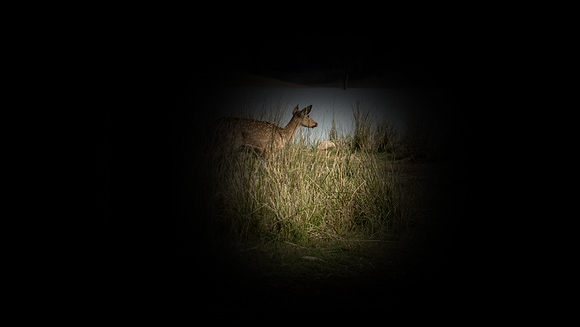
\includegraphics[width=\stepimage]{fig_poster/overview/images/h1.jpg}};
\node [pict, below=of h1, label={[align=right]left:Antelope is running\\to the right}] (h2)  {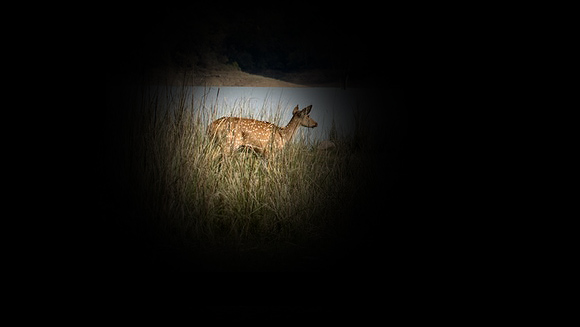
\includegraphics[width=\stepimage]{fig_poster/overview/images/h2.jpg}};
\node [pict, below=of h2, label={[align=right]left:Something orange \\is down-left}] (h3)  {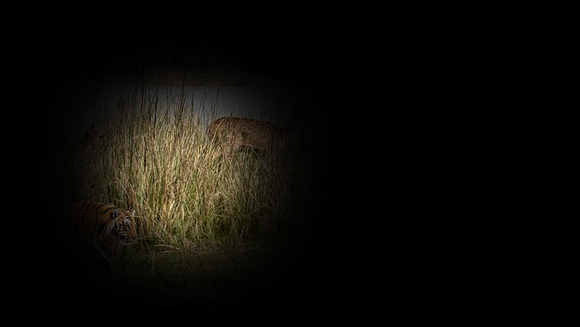
\includegraphics[width=\stepimage]{fig_poster/overview/images/h3.jpg}};
\node [pict, below=of h3, label={[align=right]left:Found a tiger!}] (h4)  {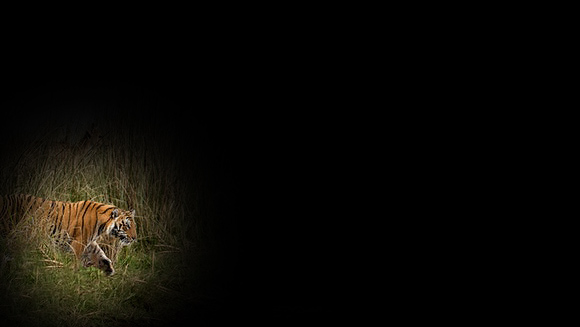
\includegraphics[width=\stepimage]{fig_poster/overview/images/h4.jpg}};

\node [pict, below=of robot, label={[align=left]right:No animal}] (r1)  {
\includegraphics[width=\stepimage]{fig_poster/overview/images/r1.jpg}};
\node [pict, below=of r1, label={[align=left]right:No animal}] (r2)  {
\includegraphics[width=\stepimage]{fig_poster/overview/images/r2.jpg}};
\node [pict, below=of r2, label={[align=left]right:No animal}] (r3)  {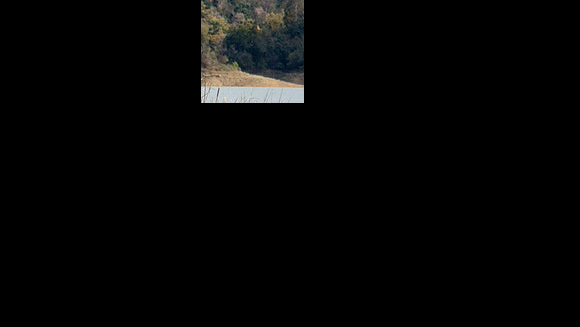
\includegraphics[width=\stepimage]{fig_poster/overview/images/r3.jpg}};
\node [inputoutput, below=of r3, label={[align=left]right:Several step later}] (r4)  {$\dotsc$};
\node [pict, below=of r4, label={[align=center]right:Not a predator}] (r5)  {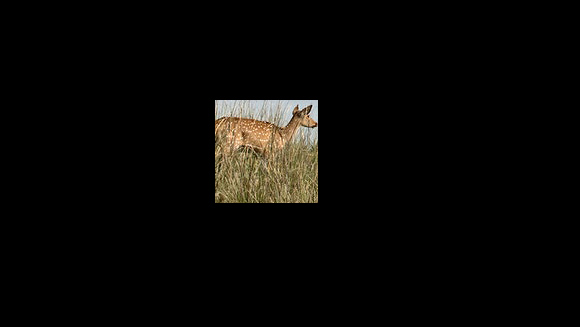
\includegraphics[width=\stepimage]{fig_poster/overview/images/r4.jpg}};
\node [inputoutput, below=of r5, label={[align=left]right:Several step later}] (r6)  {$\dotsc$};
\node [pict, below=of r6, label={[align=left]right:Found a tiger!}] (r7)  {
\includegraphics[width=\stepimage]{fig_poster/overview/images/r5.jpg}};

\draw [arrow] (task) -- (human);
\draw [arrow] (task) -- (robot);

\draw [arrow] (human) -- (h1);
\draw [arrow] (h1) -- (h2) node[midway, right] {Look left};
\draw [arrow] (h2) -- (h3) node[midway, right] {Look left};
\draw [arrow] (h3) -- (h4) node[midway, right] {Look down-left};

\draw [arrow] (robot) -- (r1);
\draw [arrow] (r1) -- (r2) node[midway, left] {Look next};
\draw [arrow] (r2) -- (r3) node[midway, left] {Look next};
\draw [arrow] (r3) -- (r4) node[midway, left] {Look next};
\draw [arrow] (r4) -- (r5) node[midway, left] {Look next};
\draw [arrow] (r5) -- (r6) node[midway, left] {Look next};
\draw [arrow] (r6) -- (r7) node[midway, left] {Look next};


\end{tikzpicture}
\end{sc}
\end{scriptsize}
\end{center}
    \caption{\textbf{Visual exploration -- human versus AI}: Humans naturally visually explore surrounding environment, using already observed areas as clues to where the wanted object can be located~\cite{hayhoe2005eye}. At the same time, common state-of-the-art artificial intelligence solutions analyze all available data, which is inefficient and waste time and computational resources. In this project, we introduce a novel Active Visual Exploration method, enabling AI agents to efficiently explore their environment.}
    \label{fig:overview}
\end{figure}

\vspace{-3.8ex}
    
\end{block}

\begin{block}{Method}
      
\begin{figure}[h]
\begin{center}
\begin{sc}
\begin{tabular}{l}
A standard approach based on auxiliary loss functions\\
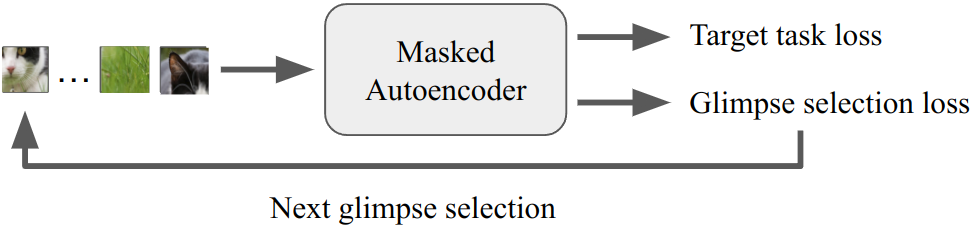
\includegraphics[scale=.6]{fig/teaser/1.png}\\[4pt]
\hline \\[\dimexpr-\normalbaselineskip+4pt]
Our approach based on internal MAE uncertainty\\
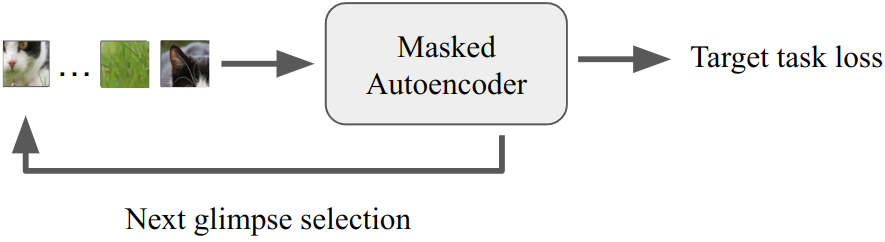
\includegraphics[scale=.6]{fig/teaser/2.png}
\end{tabular}
\end{sc}
\end{center}
\vspace{-.5ex}
\caption{\textbf{Attention-Map Entropy (AME):} Our approach chooses the most informative observations by reusing the internal uncertainty coded in the attention maps. In contrast to existing methods, it does not require any auxiliary loss functions dedicated to active exploration. Therefore, the training concentrates on the target task loss, not on an auxiliary loss, which improves overall performance.}
\label{fig:teaser}
\end{figure}


\end{block}


\end{column}

\separatorcolumn

\begin{column}{\twocolwid}

\begin{columns}[t,totalwidth=\twocolwid]

\begin{column}{\colwidth}\vspace{-2.5ex}

\begin{block}{Architecture}

\begin{figure}[t]
\vspace{.1in}
\centerline{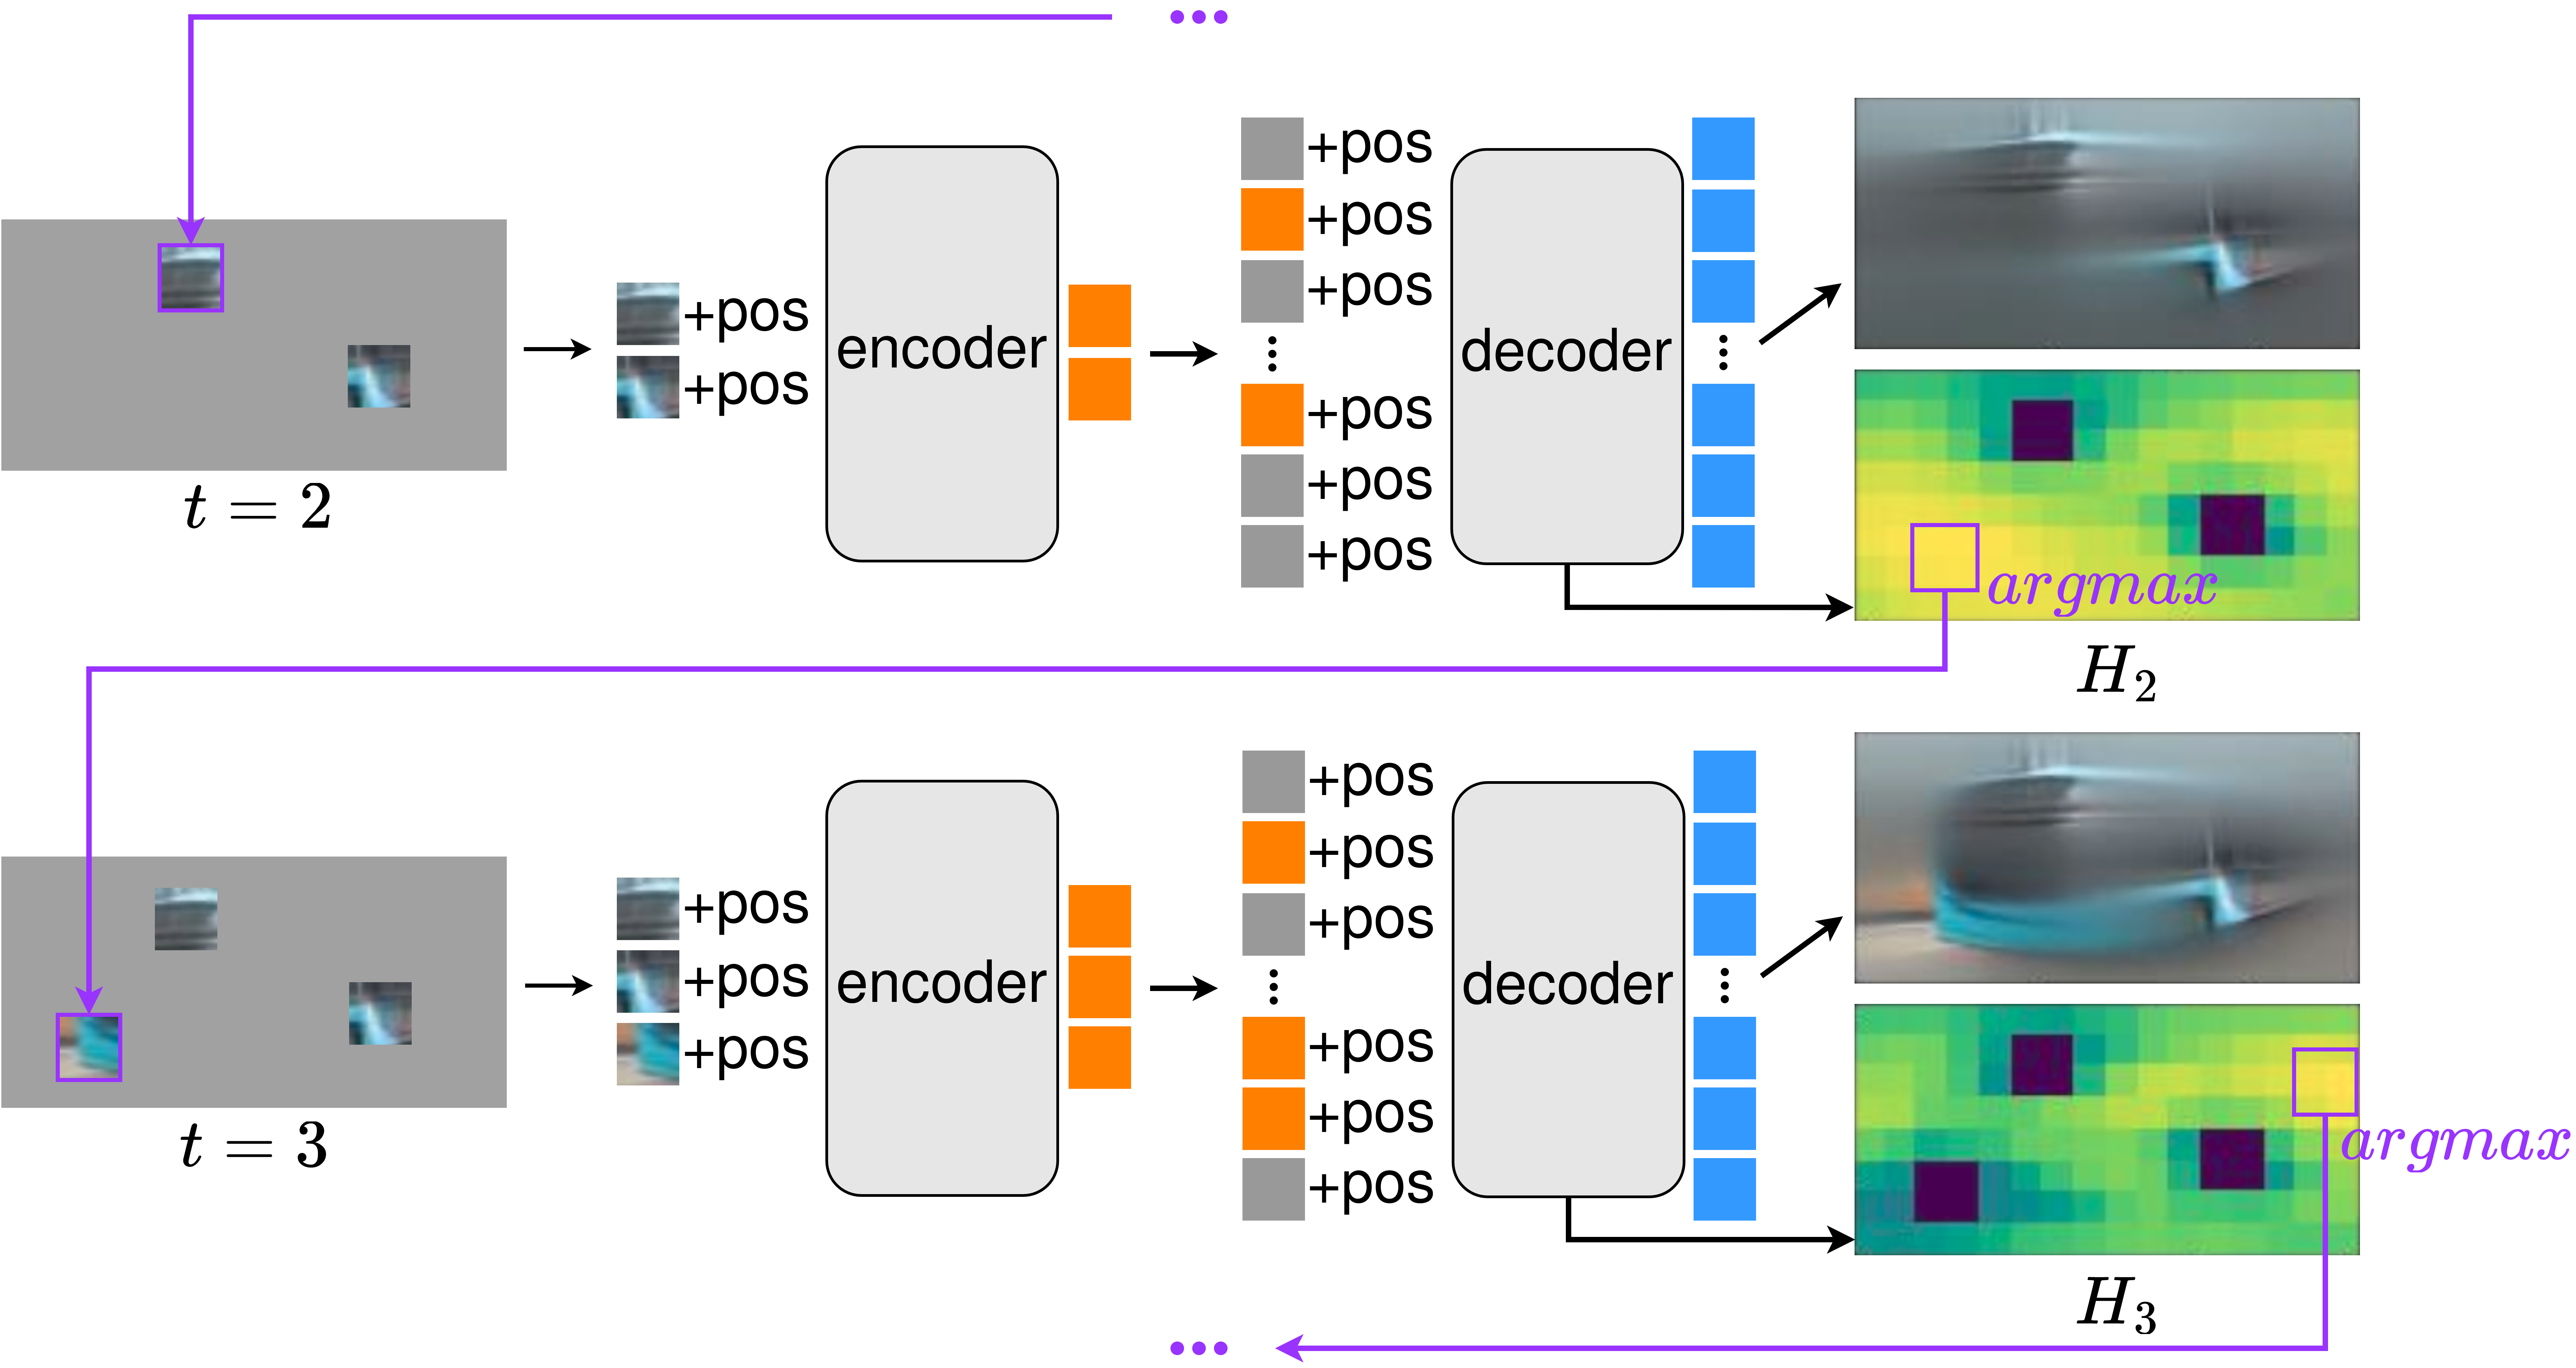
\includegraphics[width=.8\linewidth]{architecture.png}}
\caption{\textbf{Architecture for reconstruction:} The agent observed two patches of the image, which are processed by the encoder to produce their feature representations (orange rectangles). These outputs are combined with the masked patches (shown as gray rectangles) and passed through the decoder. The decoder reconstructs the missing image patches. Additionally, our method generates the entropy map for one of the decoder's multi-head self-attention layers and uses it to select the location of the third glimpse. The process repeats till we reach the assumed number of glimpses.}
\label{fig_overview}
\end{figure}
\vspace{-7ex}
    
\end{block}

\end{column}

\separatorcolumn

\begin{column}{\colwidth}\vspace{-2.5ex}

\begin{block}{Attention-map entropy}

\begin{figure}[t]
\centerline{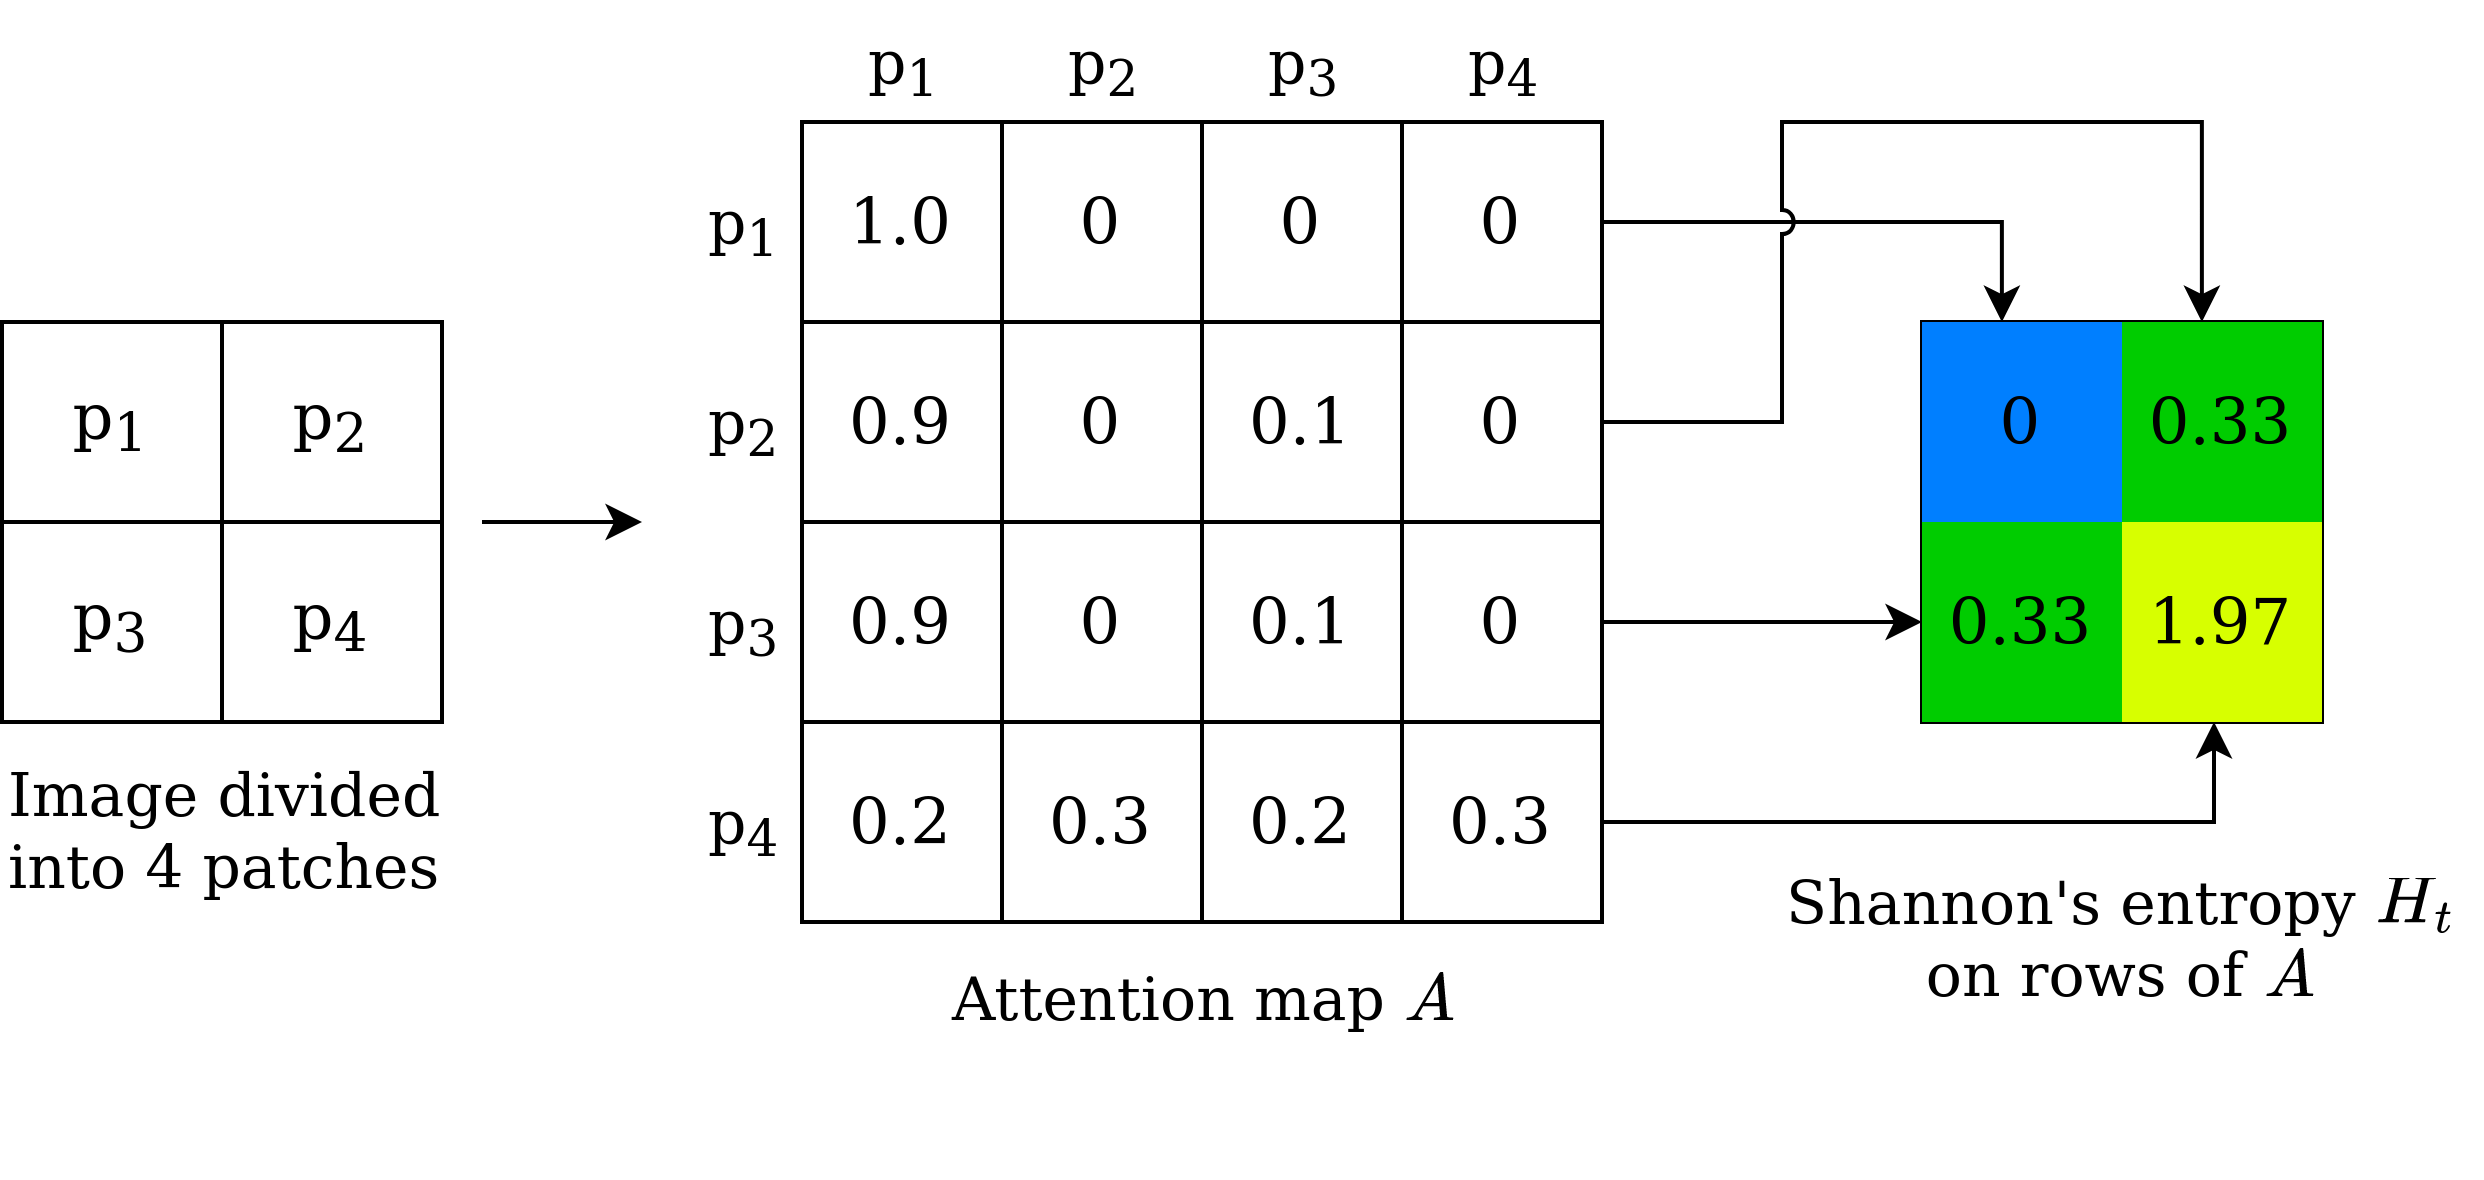
\includegraphics[width=.8\linewidth]{fig/shannon.png}}
\caption{\textbf{Entropy map:} To explain the idea of the entropy map based on attention in the transformer layer, let us consider an image divided into four patches ($2 \times 2$) on the left. Its attention map will be a $4 \times 4$ matrix, where each row represents the attention weights used to calculate the output in the next transformer layer for a corresponding patch. Calculating Shannon's entropy for each row will result in a $2 \times 2$ entropy map. The patch with the highest entropy value is selected as the next glimpse.}
\label{fig:selection}
\end{figure}
\vspace{-7ex}
    
\end{block}

\end{column}

\end{columns}


\begin{block}{Active visual exploration example}
    \begin{figure}[t]
\begin{center}
\begin{small}
\begin{sc}
\begin{tabular}{r@{\hskip2pt}c@{\hskip2pt}c@{\hskip2pt}c@{\hskip2pt}c@{\hskip2pt}c@{\hskip2pt}c@{\hskip2pt}c@{\hskip2pt}c@{\hskip2pt}|@{\hskip2pt}M{\smallimg}}
a) & 1 & 2 & 3 & 4 & 5 & 6 & 7 & 8 & \\[3pt]
b) &\tabfigure{width=\smallimg}{fig/steps/1_masked.jpg} & \tabfigure{width=\smallimg}{fig/steps/2_masked.jpg} & \tabfigure{width=\smallimg}{fig/steps/3_masked.jpg} & \tabfigure{width=\smallimg}{fig/steps/4_masked.jpg} & \tabfigure{width=\smallimg}{fig/steps/5_masked.jpg} & \tabfigure{width=\smallimg}{fig/steps/6_masked.jpg} & \tabfigure{width=\smallimg}{fig/steps/7_masked.jpg} & \tabfigure{width=\smallimg}{fig/steps/8_masked.jpg} & Ground truth\\[13pt]
c) &\tabfigure{width=\smallimg}{fig/steps/1_out.jpg} & \tabfigure{width=\smallimg}{fig/steps/2_out.jpg} & \tabfigure{width=\smallimg}{fig/steps/3_out.jpg} & \tabfigure{width=\smallimg}{fig/steps/4_out.jpg} & \tabfigure{width=\smallimg}{fig/steps/5_out.jpg} & \tabfigure{width=\smallimg}{fig/steps/6_out.jpg} & \tabfigure{width=\smallimg}{fig/steps/7_out.jpg} & \tabfigure{width=\smallimg}{fig/steps/8_out.jpg}& {\raisebox{-.28\height}{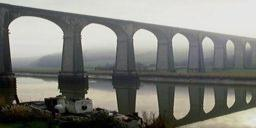
\includegraphics[width=\smallimg]{fig/steps/0_input.jpg}}}  \\[13pt]
d) &\tabfigure{width=\smallimg}{fig/steps/1_entropy.jpg} & \tabfigure{width=\smallimg}{fig/steps/2_entropy.jpg} & \tabfigure{width=\smallimg}{fig/steps/3_entropy.jpg} & \tabfigure{width=\smallimg}{fig/steps/4_entropy.jpg} & \tabfigure{width=\smallimg}{fig/steps/5_entropy.jpg} & \tabfigure{width=\smallimg}{fig/steps/6_entropy.jpg} & \tabfigure{width=\smallimg}{fig/steps/7_entropy.jpg} &&
\end{tabular}
\end{sc}
\end{small}
\end{center}
\vskip -0.1in
\caption{\textbf{Glimpse-based reconstruction step-by-step:} The figure shows a glimpse selection process based on AME for $8\times32^2$ glimpses for a sample $256\times128$ image. The rows correspond to \textsc{a)} step number, \textsc{b)} model input (glimpses), \textsc{c)} model prediction given, \textsc{d)} decoder attention entropy (known areas are explicitly set to zero). The algorithm explores the image in places where the reconstruction result is blurry.}
\label{fig:steps}
\end{figure}
\vspace{-4ex}
\end{block}


\begin{block}{Results}

\begin{columns}[t,totalwidth=\twocolwid]

\begin{column}{\colwidth}

\vspace{-3ex}
\begin{table}[t]
\begin{center}
\begin{sc}
\begin{footnotesize}
\begin{tabular}{l@{}rrrllrr}
\toprule
Method & SUN360 & ADE20k & MSCOCO & Image res. & Glimpse regime & Pixel \% & Area \% \\
\midrule
AttSeg & 37.6 & 36.6 & 41.8 & $128 \times 256$ & $8 \times 48^2$ (retinal) & 18.75 & 56.25 \\
GlAtEx & 33.8 & 41.9 & 40.3 & $128 \times 256$ & $8 \times 48^2$ (retinal) & 18.75 & 56.25 \\
Ours (retinal) & \textbf{23.6} & \textbf{23.8} & \textbf{25.2} & $128 \times 256$ & $8 \times 48^2$ (retinal) & 18.75 & 56.25\\
\midrule
Ours (non-retinal) & 37.9 & 40.7 & 43.2 & $128 \times 256$ & $8 \times 16^2$ (non ret.) & 6.25 & 6.25\\
Ours (non-retinal) & 29.8 & 30.8 & 32.5 & $128 \times 256$ & $8 \times 32^2$ (non ret.) & 25.00 & 25.00\\
Ours (non-retinal) & \textbf{20,1} & \textbf{20.6} & \textbf{22.1} & $128 \times 256$ & $8 \times 48^2$ (non ret.) & 56.25 & 56.25 \\
\midrule
SimGlim (detached) & 26.2 & 27.2 & 29.8 & $224 \times 224$ & $37 \times 16^2$ (non ret.) & 18.75 & 18.75\\
SimGlim (end-to-end) & 28.0 & 28.8 & 31.3 & $224 \times 224$ & $37 \times 16^2$ (non ret.) & 18.75 & 18.75 \\
Ours (non-retinal) & \textbf{23.4} & \textbf{26.2} & \textbf{28.6} & $224 \times 224$ & $37 \times 16^2$ (non ret.) & 18.75 & 18.75 \\
\bottomrule
\end{tabular}
\end{footnotesize}
\end{sc}
\end{center}
\caption{\textbf{Reconstruction results:} Comparison of our model in reconstruction task against AttSeg~\protect\cite{seifi2020segment}, GlAtEx~\protect\cite{seifi2021glimpse} and SimGlim~\protect\cite{Jha2023WACV} on SUN360~\cite{song2015sun}, ADE20K~\cite{zhou2017scene} and MS~COCO~\cite{lin2014microsoft} datasets. The metric used is a root mean square error (RMSE; lower is better). For each experiment, we provide a training and evaluation regime defined by a number of glimpses of a specific resolution. Pixel \% and area \% denote respectively: the percentage of image pixels known to the model and the percentage of image area seen by the model. Differences in both measures occur when dealing with retina-like glimpses, which have lower pixel counts by design. Our method outperforms competitive solutions in all configurations.}
\label{tab:reconstruction}
\end{table}
% \vspace{-1ex}

\begin{figure}[t]
\begin{center}
\begin{small}
\begin{sc}
\begin{tabular}{c@{\hskip2pt}c@{\hskip2pt}c@{\hskip2pt}c}
Input&Ours&GlAtEx&AttSeg\\
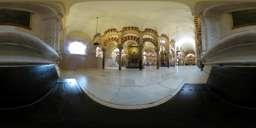
\includegraphics[width=\smallimg]{fig/sun360/1/gt.jpg}&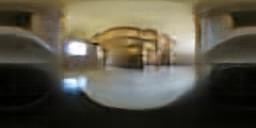
\includegraphics[width=\smallimg]{fig/sun360/1/ours.jpg}&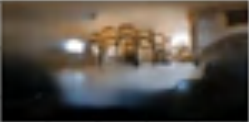
\includegraphics[width=\smallimg]{fig/sun360/1/glatex.png}&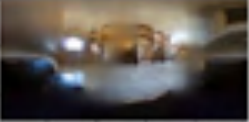
\includegraphics[width=\smallimg]{fig/sun360/1/atseg.png}\\

\includegraphics[width=\smallimg]{fig/sun360/2/gt.jpg}&
\includegraphics[width=\smallimg]{fig/sun360/2/ours.jpg}&
\includegraphics[width=\smallimg]{fig/sun360/2/glatex.png}&
\includegraphics[width=\smallimg]{fig/sun360/2/atseg.png}\\

\includegraphics[width=\smallimg]{fig/sun360/3/gt.jpg}&
\includegraphics[width=\smallimg]{fig/sun360/3/ours.jpg}&
\includegraphics[width=\smallimg]{fig/sun360/3/glatex.png}&
\includegraphics[width=\smallimg]{fig/sun360/3/atseg.png}\\

\includegraphics[width=\smallimg]{fig/sun360/5/gt.jpg}&
\includegraphics[width=\smallimg]{fig/sun360/5/ours.jpg}&
\includegraphics[width=\smallimg]{fig/sun360/5/glatex.png}&
\includegraphics[width=\smallimg]{fig/sun360/5/atseg.png}\\
\end{tabular}
\end{sc}
\end{small}
\end{center}
\vskip -0.1in
\caption{\textbf{Reconstruction quality for SUN360:} Reconstruction results of our method compared with AttSeg~\protect\cite{seifi2020segment} and GlAtEx~\protect\cite{seifi2021glimpse} on the SUN360 dataset. Reconstructions done with our method are visibly better than the competition.}
\label{fig:qualiative-retinal}
\end{figure}


\end{column}

\separatorcolumn

\begin{column}{\colwidth}

\begin{figure}[t]
\begin{center}
\begin{small}
\begin{sc}
\begin{tabular}{c@{\hskip2pt}c@{\hskip2pt}c|c@{\hskip2pt}c@{\hskip2pt}c}
Input&Ours&SimGlim&Input&Ours&SimGlim\\

\includegraphics[width=\smallerimg]{fig/ade/3/gt.jpg}&
\includegraphics[width=\smallerimg]{fig/ade/3/ours.jpg}&
\includegraphics[width=\smallerimg]{fig/ade/3/simglim.png}&

\includegraphics[width=\smallerimg]{fig/ade/2/gt.jpg}&
\includegraphics[width=\smallerimg]{fig/ade/2/ours.jpg}&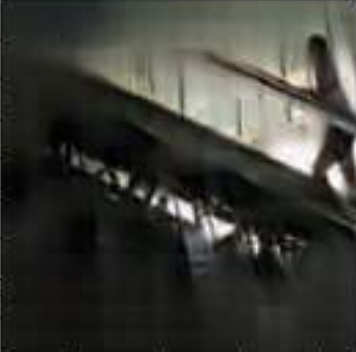
\includegraphics[width=\smallerimg]{fig/ade/2/simglim.png}\\

\includegraphics[width=\smallerimg]{fig/ade/4/gt.jpg}&
\includegraphics[width=\smallerimg]{fig/ade/4/ours.jpg}&
\includegraphics[width=\smallerimg]{fig/ade/4/simglim.png}&

\includegraphics[width=\smallerimg]{fig/ade/5/gt.jpg}&
\includegraphics[width=\smallerimg]{fig/ade/5/ours.jpg}&
\includegraphics[width=\smallerimg]{fig/ade/5/simglim.png}\\
\end{tabular}
\end{sc}
\end{small}
\end{center}
\vskip -0.1in
\caption{\textbf{Reconstruction quality for ADE20K:} Figure shows difference in reconstruction quality against SimGlim~\protect\cite{Jha2023WACV} on the ADE20K dataset. SimGlim reconstructs a single object slightly better, but our method recovers more objects in the scene.}
\label{fig:qualiative-non-retinal}
\end{figure}


\begin{columns}[t, totalwidth=\colwidth]

\begin{column}{.47\colwidth}

\begin{table}[t]
\begin{center}
\begin{sc}
\begin{footnotesize}
\begin{tabular}{cccc}
\toprule
Method & mPA(\%) & PA(\%) & IoU(\%) \\
\midrule
AttSeg & - & 47.9 & -\\
GlAtEx & - & 52.4 & -\\
Ours (MAE-weights) & 32.2 & \textbf{70.27} & 24.4\\
Ours (SETR-weights) & \textbf{35.6} & 69.5 & \textbf{27.6}\\
\bottomrule
\end{tabular}
\end{footnotesize}
\end{sc}
\end{center}
\vskip -0.1in
\caption{\textbf{Segmentation results:} Comparison of our model against AttSeg~\protect\cite{seifi2020segment} and GlAtEx~\protect\cite{seifi2021glimpse}. The metric used is mean Pixel-wise Accuracy (mPA, higher is better), Pixel-Accuracy (PA, higher is better), and Intersection over Union (IoU, higher is better). Our solution outperforms competitive methods on all metrics.}
\label{tab:segmentation}
\end{table}

\end{column}
\begin{column}{.02\textwidth}\end{column}
\begin{column}{.47\colwidth}

\begin{table}[t]
\begin{center}
\begin{sc}
\begin{footnotesize}
\begin{tabular}{lr}
\toprule
Method & Accuracy (\%) \\
\midrule
AttSeg & 52.6\\
GlAtEx (full) & 56.4\\
GlAtEx (no decoder) & 67.2\\
Ours (head-only) & 70.1\\
Ours (train-all) & \textbf{75.7}\\
\bottomrule
\end{tabular}
\end{footnotesize}
\end{sc}
\end{center}
\vskip -0.1in
\caption{\textbf{Classification results:} Comparison of our model's classification performance against AttSeg~\protect\cite{seifi2020segment} and GlAtEx~\protect\cite{seifi2021glimpse} on the SUN360 dataset. The metric used is accuracy (higher is better). Our method outperforms competitive methods in both Train-all and Head-only training options.}
\label{tab:classification}
\end{table}
\vspace{-3ex}

\end{column}
\end{columns}


\end{column}

\end{columns}

\end{block}

\end{column}


\separatorcolumn

\begin{column}{\colwidth}
\begin{block}{Results cont.}

\begin{figure}[t]
\begin{center}
\begin{small}
\begin{sc}
\begin{tabular}{c@{\hskip2pt}c@{\hskip2pt}c@{\hskip2pt}c}
Image&Target&Ours&GlAtEx\\
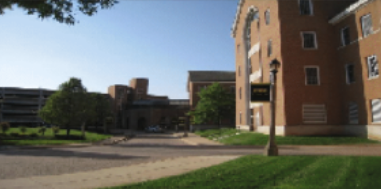
\includegraphics[width=\smallimg]{fig/seg/1/img.png}&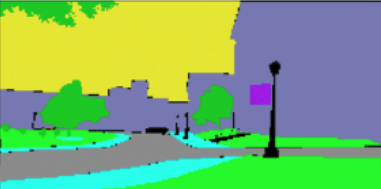
\includegraphics[width=\smallimg]{fig/seg/1/gt.png}&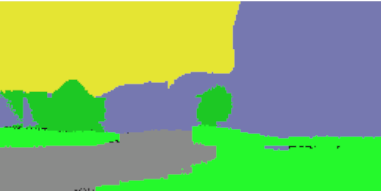
\includegraphics[width=\smallimg]{fig/seg/1/ours.png}&
\includegraphics[width=\smallimg]{fig/seg/1/glatex.png}\\

\includegraphics[width=\smallimg]{fig/seg/2/img.png}&
\includegraphics[width=\smallimg]{fig/seg/2/gt.png}&
\includegraphics[width=\smallimg]{fig/seg/2/ours.png}&
\includegraphics[width=\smallimg]{fig/seg/2/glatex.png}\\

\includegraphics[width=\smallimg]{fig/seg/3/img.png}&
\includegraphics[width=\smallimg]{fig/seg/3/gt.png}&
\includegraphics[width=\smallimg]{fig/seg/3/ours.png}&
\includegraphics[width=\smallimg]{fig/seg/3/glatex.png}\\

\includegraphics[width=\smallimg]{fig/seg/4/img.png}&
\includegraphics[width=\smallimg]{fig/seg/4/gt.png}&
\includegraphics[width=\smallimg]{fig/seg/4/ours.png}&
\includegraphics[width=\smallimg]{fig/seg/4/glatex.png}\\
\end{tabular}
\end{sc}
\end{small}
\end{center}
\vskip -0.1in
\caption{\textbf{Segmentation quality for ADE20K:} Semantic segmentation results of our method compared with GlAtEx~\protect\cite{seifi2021glimpse} on the ADE20k dataset. Qualitatively, segmentation maps produced by our method are at least as good as those of the competition.}
\label{fig:qualiative-seg}
\end{figure}
\vspace{-4ex}

\end{block}


\begin{block}{Acknowledgments}
\footnotesize{
    This research was funded by National Science Centre, Poland (grants no 2020/39/B/ST6/01511, 2022/45/B/ST6/02817, and 2021/41/B/ST6/01370), Foundation for Polish Science (grant no POIR.04.04.00-00-14DE/18-00 carried out within the Team-Net program co-financed by the European Union under the European Regional Development Fund). We gratefully acknowledge Polish high-performance computing infrastructure PLGrid (HPC Centers: ACK Cyfronet AGH) for providing computer facilities and support within computational grant no. PLG/2022/015753. The research was supported by a grant from the Faculty of Mathematics and Computer Science under the Strategic Programme Excellence Initiative at Jagiellonian University.
    }
\vspace{-2ex}
\end{block}

\begin{block}{References}
\vspace{-.5ex}
    \footnotesize{\bibliographystyle{plain}\bibliography{example_paper}}
    \vspace{-.5ex}
  \end{block}
\begin{block}{Read the paper at}
\begin{center}
\vspace{-3ex}

\includegraphics[height=20ex]{fig/logos/qr.png}
\vspace{-4ex}
\end{center}
\end{block}
\begin{block}

\begin{center}
\vspace{-2ex}

\begin{tikzpicture}[node distance=4ex, auto]
\tikzstyle{pict} = [inner sep=0px]

\node[pict] (ideas) {
\includegraphics[width=.25\linewidth]{fig/logos/ideas.png}};

\node[pict, right=2em of ideas, yshift=1ex] (uj) {
\includegraphics[width=.25\linewidth]{fig/logos/uj.png}};

\node[pict, right=2em of uj, yshift=-1ex] (pw) {
\includegraphics[width=.28\linewidth]{fig/logos/pw.png}};

\node[pict, below=of ideas] (gmum) {
\includegraphics[width=.25\linewidth]{fig/logos/gmum.png}};

\node[pict] at (gmum -| pw) (tooploox) {
\includegraphics[width=.28\linewidth]{fig/logos/tooploox.png}};

\node[pict] (ardigen) at (gmum -| uj) {
\includegraphics[width=.25\linewidth]{fig/logos/ardigen.png}};

\node[pict, above=of uj, yshift=-2ex] (ijcai) {
\includegraphics[width=.38\linewidth]{fig/logos/ijcai-logo.png}};

\end{tikzpicture}
\end{center}
    
\end{block}
  
\end{column}

\separatorcolumn


\end{columns}
\end{frame}

\end{document}
